
\subsection{Resistencia de entrada}

\begin{itemize}
	
	\HgraficarEPS{0.5}{ri}{Diagrama en bloque para hallar la resistencia de entrada.}{fig.esq_ri}
		
\item \textbf{Resistencia de entrada sin realimentación}
	
	\begin{equation}
		\centering
		R_{i,SR} = \SI{100}{\ohm} + R_{F1}//R_{F2} = \SI{100}{\ohm} + \SI{22}{\kilo\ohm}//\SI{1.1}{\kilo\ohm}
	\end{equation}
	
\item \textbf{Resistencia de entrada con realimentación}
	\HgraficarEPS{0.5}{ri_realim}{Diagrama en bloque para hallar la resistencia de entrada.}{fig.esq_ri_f}
	\begin{equation}
		\centering
		R_{i,CR} = (1+ af) \cdot R_{i,SR} = (1 + 1485) \cdot \SI{1.1}{\kilo\ohm} = \SI{1.6}{\mega\ohm}
	\end{equation}
	
\end{itemize}

Finalmente la resistencia que ve el generador es

$$ \SI{100}{\kilo\ohm}//\SI{1.6}{\mega\ohm} = \boxed{\SI{94}{\kilo\ohm}} $$


\subsection{Impedancia de salida}

\begin{figure}[H]
	 \centering
	 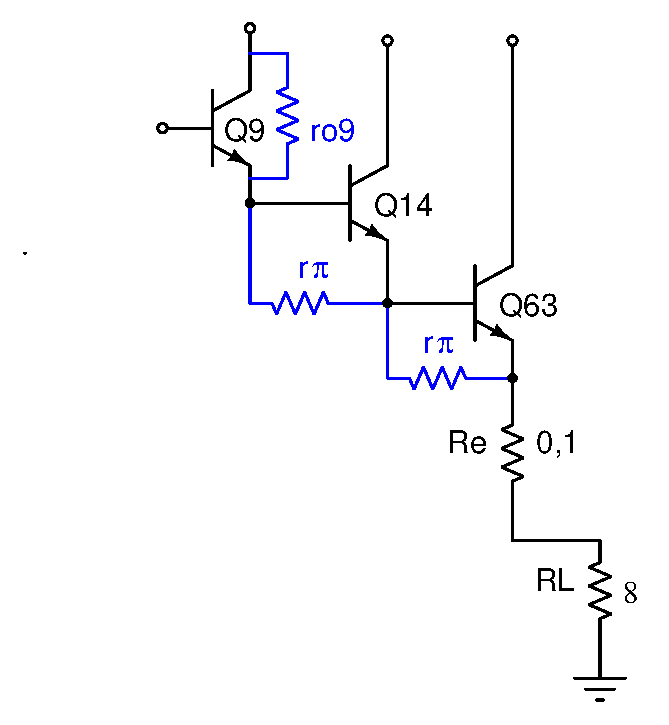
\includegraphics[scale=0.5]{ro.eps}
	 \caption{Diagrama para hallar la resistencia de salida del circuito sin realimentación.}
\end{figure}

\begin{itemize}
	\item Resistencia de salida sin realimentador: en esta situación se supone que, a los efectos de este cálculo, las resistencias de salida de los colectores comunes son iguales.
Entonces se calcula la resistencia de salida del circuito sin realimentar como
	\begin{equation}
		\centering
		R_o = \frac{1}{2} \cdot R_E + \frac{ r_{\pi}^{*} + r_{o,Q9} }{\beta^{*} } = \frac{1}{2} \left ( \SI{0.1}{\ohm} + \frac{\SI{32}{\kilo\ohm}}{75 \cdot 60} \right) = \SI{3.6}{\ohm}
	\end{equation}
	siendo
	\begin{equation}
		\centering
		r_{\pi}^{*} = 2 \cdot r_{\pi_{Q_{14}}} = 2 \cdot 60 \cdot \frac{25mV}{ \SI{110}{\milli\ampere}} = \SI{14}{\ohm} 
	\end{equation}
		
	%\begin{equation}
	%	\centering
	%	r_{o,Q9} = \frac{160V}{5mA} = \SI{32}{\kilo\ohm}
	%\end{equation}
		
	\item Resistencia de salida con realimentador
	\begin{equation}
		\centering
		R_{o,CR} = \frac{R_{o,SR}}{1+ af} = \frac{ \SI{3.6}{\ohm} }{1+1485} = \boxed{\SI{2.4}{\milli\ohm}} 
	\end{equation}
\end{itemize}

\subsection{Factor de amortiguamiento}

En un sistema de audio, el factor de amortiguamiento es la relación entre la impedancia del altoparlante y la impedancia de salida del amplificador. Describe la capacidad del amplificador de controlar movimiento del altoparlante cuando se deja de excitarlo, en especial cercano a su frecuencia de resonancia. Este valor es de importancia en el contexto de las bajas frecuencias, o subwoofers, dado que la inercia de los diafragmas suele ser grande y el control de la suspensión débil, para permitir grandes excursiones.

\begin{equation}
	\centering
	f_a= \frac{Z_L}{Z_o} = \frac{ \SI{8}{\ohm}}{ \SI{2.4}{\milli\ohm}}= \boxed{\num{3333}}
	\label{ec:fa}
\end{equation}



